\documentclass[10pt,a4paper]{llncs}

\frontmatter
\usepackage{cmap}

\usepackage[greek,english]{babel}
\languageattribute{greek}{polutoniko}
\usepackage{hyperref}
\addto\extrasenglish{\def\figureautorefname{figure}}
\addto\extrasenglish{\def\subsectionautorefname{section}}
\addto\extrasenglish{\def\subsubsectionautorefname{section}}

\usepackage{amsmath,amssymb}
\usepackage{lmodern}
\usepackage{stmaryrd}
\usepackage{comment}
\usepackage{ifthen}
\usepackage{makeidx}

\usepackage{bussproofs}
\usepackage{graphicx}
\EnableBpAbbreviations
\usepackage{mdframed}
\newenvironment{scprooftree}[1]%
  {\gdef\scalefactor{#1}\begin{center}\proofSkipAmount \leavevmode}%
  {\scalebox{\scalefactor}{\DisplayProof}\proofSkipAmount \end{center} }
\newenvironment{scprooftree*}[1]%
  {\gdef\scalefactor{#1} \leavevmode\hbox\bgroup}%
  {\scalebox{\scalefactor}{\DisplayProof} \egroup}

\usepackage{natbib}
\usepackage{etoolbox}
\usepackage{xstring}
\makeatletter
\patchcmd{\NAT@test}{\else \NAT@nm}{\else \NAT@nmfmt{\NAT@nm}}{}{}

\DeclareRobustCommand\citepos
  {\begingroup
   \let\NAT@nmfmt\NAT@posfmt% ...except with a different name format
   \NAT@swafalse\let\NAT@ctype\z@\NAT@partrue
   \@ifstar{\NAT@fulltrue\NAT@citetp}{\NAT@fullfalse\NAT@citetp}}

\let\NAT@orig@nmfmt\NAT@nmfmt
\def\NAT@posfmt#1{%
  \StrRemoveBraces{#1}[\NAT@temp]%
  \IfEndWith{\NAT@temp}{s}
    {\NAT@orig@nmfmt{#1'}}
    {\NAT@orig@nmfmt{#1's}}}
\makeatother
\newcommand{\mathplus}[0]{+}

% abbrev.
\def\NLIBC{NL$_{\text{IBC}}$}
\def\I{\ensuremath{\mathbf{I}}}
\def\B{\ensuremath{\mathbf{B}}}
\def\C{\ensuremath{\mathbf{C}}}
\def\Q{\ensuremath{\mathbf{Q}}}

% only during writing
\usepackage{xcolor}


\begin{document}

\mainmatter%
\title{Strong and weak quantifiers in focused \NLCL}
%\author{Pepijn Kokke}
%\institute{%
%  Institute for Logic, Language and Computation\\
%  University of Amsterdam, Amsterdam\\
%  \email{pepijn.kokke@gmail.com}}
\maketitle

\section{Introduction}\label{sec:introduction}

In \citeyear{kiselyov2014}, \citet{kiselyov2014} published a
paper in which they presented an elegant approach to the anaysis of
various scope-related phenomena using, what they call, the
continuation hierarchy.
The phenomena they cover are scope ambiguity, scope islands and strong
and weak quantifiers.
They cover these phenomena using a mechanism which works on the
sentence's \emph{semantics}, independent of whatever form of grammar
is used.

At around the same time, \citepos{barker2015} published a book
containing their findings on {\NLLAM} and {\NLCL}, a pair of grammar
logics, both with the ability to analyse scope ambiguity using a
strictly \emph{syntactic} mechanism.
In addition, these logics can analyse ``parastic scope''
\citep{barker2007,barker2015} and a quantifiers which change the
result type of the expressions they take scope over.
However, neither of these logics is capable of analysing scope islands
or strong and weak quantifiers.

In this paper, we rework {\NLCL} to a calculus which can analyse both
scope islands and strong and weak quantifiers, without losing
the ability to analyse parasitic scope or changing result types.
We base ourselves on work by \citet{moortgat1996} and
\citet{moortgat2012}. As a bonus, our approach to strong and weak
quantifiers requires a focusing regime. This results in the elimination
of spurious ambiguity, and thus greatly enhances the efficiency of
proof search.

We will start our discussion by giving several examples of each of the
aforementioned phenomena. The following sentences are examples of scope
ambiguity, scope islands and weak quantifiers, respectively. They are
given together with their expected semantics, and are based on
examples by \citet[][p.\ 608, 622]{szabolcsi2000}.
\eenumsentence{\label{ex:scope-ambiguity}
\item[]\hspace*{-0.5\leftmargin}%
  ``Someone read every book.''
\item%
  \(
  \exists{x}.\PERSON(x)\wedge\forall{y}.\BOOK(y)\supset\READ(x,y)
  \)
\item%
  \(
  \forall{y}.\BOOK(y)\supset\exists{x}.\PERSON(x)\wedge\READ(x,y)
  \)}
\eenumsentence{\label{ex:scope-island}
\item[]\hspace*{-0.5\leftmargin}%
  ``Someone said Kurt wrote every book.''
\item%
  \(
  \exists{x}.\PERSON(x)\wedge\SAY(x,\forall{y}.\BOOK(y)\supset\WROTE(\KURT,y))
  \)}
\eenumsentence{\label{ex:weak-quantifier}
\item[]\hspace*{-0.5\leftmargin}%
  ``Everyone said [Kurt dedicated a book to Mary].''
\item%
  \(
  \forall{x}.\PERSON(x)\supset\SAY(x,\exists{y}.\BOOK(y)
  \wedge\DEDICATE(\KURT,\MARY,y))
  \)
\item%
  \(
  \forall{x}.\PERSON(x)\supset\exists{y}.\BOOK(y)
  \wedge\SAY(x,\DEDICATE(\KURT,\MARY,y))
  \)
\item%
  \(
  \exists{y}.\BOOK(y)
  \wedge\forall{x}.\PERSON(x)\supset\SAY(x,\DEDICATE(\KURT,\MARY,y))
  \)}
The first of these examples is a canonical example of scope
ambiguity.
%
Example (\ref{ex:scope-island}) demonstrates a scope
island: there is no reading in which ``every book'' scopes out of the
embedded clause, as this reading would imply that the speaker made a
separate speech act for every book: ``Kurt wrote
Slaughterhouse-Five'', ``Kurt wrote Cat's Cradle'', ``Kurt
wrote\ldots''
%
Finally, example (\ref{ex:weak-quantifier}) shows that
indefinites \emph{can} scope out of scope islands.

We add two more sentences, which are examples of a quantifier which
changes the result type, and of parasitic scope, respectively. These
examples based on those given by \citepos[][p.\ 208]{barker2015} and
\citet{kiselyov2015b}.
\eenumsentence{\label{ex:changing-result-type}
\item[]\hspace*{-0.5\leftmargin}%
  ``John read a book [the author of which] feared the ocean.''
\item%
  \(
  \exists{x}.\BOOK(x)
  \wedge\FEAR(\iota(\lambda{y}.\OF(y,\AUTHOR,x)),\iota(\OCEAN))
  \wedge\READ(\JOHN,x)
  \)}
\eenumsentence{\label{ex:parasitic-scope}
\item[]\hspace*{-0.5\leftmargin}%
  ``Everyone feared the same ocean.''
\item%
  \(
  \exists{z}.\forall{y}.\FEAR(y,\iota(\lambda{x}.\OCEAN(x)\wedge{x=z}))
  \)}
These last two examples will play a less important role, as {\NLCL} is
already capable of analysing both. However, in order to demonstrate
that we have not lost that capability, we will provide analyses of
both near the end of this paper.

\section{Background}
In this section, we will briefly discuss {\NLCL} and its sibling,
{\NLLAM}. {\NLCL} is an extension to the non-associative Lambek
calculus \citep[NL;][]{lambek1961}.
The history behind {\NLCL} is somewhat intricate, but helpful to
understanding, so we will briefly go over it.
The initial idea comes from the practice of encoding quantifier
movement as a tree transformation which introduces a
binder~\citep{heim1998}:
\begin{center}
  \begin{minipage}{0.4\linewidth}\centering
    \begin{tikzpicture}
      \tikzset{level distance=4ex}
      \tikzset{sibling distance=0pt}
      \Tree [ john [ likes everyone ] ]
    \end{tikzpicture}
  \end{minipage}%
  \begin{minipage}{0.05\linewidth}\centering
    $\longleftrightarrow$
  \end{minipage}%
  \begin{minipage}{0.5\linewidth}\centering
    \begin{tikzpicture}
      \tikzset{level distance=4ex}
      \tikzset{sibling distance=0pt}
      \Tree [ everyone [ $\lambda x.$ [ john [ likes $x$ ] ] ] ]
    \end{tikzpicture}
  \end{minipage}
\end{center}
To implement this idea in type-logical grammar,
\citeauthor{barker2015} add a structural $\lambda$-construct to NL,
and added the following structural postulate:\footnote{%
  It is important to note that this construct is \emph{purely
  structural}, and that it is not accompanied by some implicit form of
  computation (e.g.\ $\beta,\eta$-conversions).
}
\begin{align}
  \tag{$\lambda$}
  \Sigma[\Gamma] \longleftrightarrow \Gamma\hprod\lambda{x}.\Sigma[x]
  \label{eqn:lambda}
\end{align}
As can be seen, the~\eqref{eqn:lambda} postulate uses a new
connective: the $\hprod$ (hollow product).
This connective is part of a new residuated family $\{\himpr, \hprod,
\himpl\}$, which starts out as a copy of $\{\impr, \prod,
\impl\}$.
However, the addition of the~\eqref{eqn:lambda} postulate allows you
to raise any constituent to the top-left position in the structure,
where---if it has the right type---it can be ``resolved'' against the
top-level type as follows:
\begin{scprooftree}
  \AXC{$\Sigma[{A}]\fCenter{B}$}
  \RightLabel{\eqref{eqn:lambda}}
  \UIC{${A}\hprod\lambda{x}.\Sigma[x]\fCenter{B}$}
  \RightLabel{R$\himpr$}
  \UIC{$\lambda{x}.\Sigma[x]\fCenter{A\himpr B}$}
  \AXC{${C}\fCenter{D}$} \RightLabel{L$\himpl$}
  \BIC{${C\himpl(A\himpr B)}\hprod\lambda{x}.\Sigma[x]\fCenter{D}$}
  \RightLabel{\eqref{eqn:lambda}}
  \UIC{$\Sigma[{C\himpl(A\himpr B)}]\fCenter{D}$}
\end{scprooftree}
\citeauthor{barker2015} call resulting system {\NLLAM}.
While {\NLLAM} fulfils the promise of allowing a syntactic analysis of
quantifier raising, scope ambiguity and parasitic scope, it has some
problems.
Most notably, the system is hard to formalise and to reason about,
largely due to the presence of a binding construct in the syntax of
structures.
While it is not impossible to formalise, the~\eqref{eqn:lambda}
postulate greatly complicates meta-logical proofs.

To address this issue, and to ease their own investigation of the
formal properties of {\NLLAM}, \citet[][ch.\ 17]{barker2015} introduce
{\NLCL}.
This system uses the fact that $\lambda$-terms can be represented as
combinators in combinatory logic, which removes the need for a binding
construct.
\citeauthor{barker2015} use a variant of Sch\"onfinkel's mapping to
encode the \emph{linear} $\lambda$-construct as applications of the
combinators $\I$, $\B$ and $\C$:\footnote{%
  One can easily verify that the $\lambda$-construct introduced
  by~\eqref{eqn:lambda} is linear.
}\footnote{%
  When comparing these equations to the \I\B\C-rules in
  \autoref{fig:nlcl}, note that $\prod$ encodes function application,
  but $\hprod$ encodes \emph{flipped} function application.
}
\[
  \I x     = x,
  \qquad
  \B x y z = x (y z),
  \qquad
  \C x y z = x  z y
\]
The resulting system is presented in \autoref{fig:nlcl}.\footnote{%
  In \autoref{fig:nlcl}, and for the remainder of this paper, the
  letters $\Gamma$ and $\Delta$ are reserved for structures, whereas
  the $\Sigma$ is used for contexts.
}

\begin{figure}[h!]
  \centering

  \begin{scprooftree*}
    \AXC{}\RightLabel{Ax}\UIC{$A\fCenter A$}
  \end{scprooftree*}

  \vspace*{1\baselineskip}
  \begin{scprooftree*}
    \AXC{$\Gamma\fCenter A$}
    \AXC{$\Sigma[B]\fCenter C$}
    \RightLabel{$\impr L$}
    \BIC{$\Sigma[\Gamma\prod A\impr B]\fCenter C$}
  \end{scprooftree*}%
  \begin{scprooftree*}
    \AXC{$A\prod\Gamma\fCenter B$}
    \RightLabel{$\impr R$}
    \UIC{$\Gamma\fCenter A\impr B$}
  \end{scprooftree*}%
  \begin{scprooftree*}
    \AXC{$\Gamma\fCenter A$}
    \AXC{$\Sigma[B]\fCenter C$}
    \RightLabel{$\impl L$}
    \BIC{$\Sigma[B\impl A \prod\Gamma]\fCenter C$}
  \end{scprooftree*}%
  \begin{scprooftree*}
    \AXC{$\Gamma\prod A\fCenter B$}
    \RightLabel{$\impl R$}
    \UIC{$\Gamma\fCenter B\impl A$}
  \end{scprooftree*}

  \vspace*{1\baselineskip}
  \begin{scprooftree*}
    \AXC{$\Gamma\fCenter A$}
    \AXC{$\Sigma[B]\fCenter C$}
    \RightLabel{$\himpr L$}
    \BIC{$\Sigma[\Gamma\hprod A\himpr B]\fCenter C$}
  \end{scprooftree*}%
  \begin{scprooftree*}
    \AXC{$A\hprod\Gamma\fCenter B$}
    \RightLabel{$\himpr R$}
    \UIC{$\Gamma\fCenter A\himpr B$}
  \end{scprooftree*}%
  \begin{scprooftree*}
    \AXC{$\Gamma\fCenter A$}
    \AXC{$\Sigma[B]\fCenter C$}
    \RightLabel{$\himpl L$}
    \BIC{$\Sigma[B\himpl A \hprod\Gamma]\fCenter C$}
  \end{scprooftree*}%
  \begin{scprooftree*}
    \AXC{$\Gamma\hprod A\fCenter B$}
    \RightLabel{$\himpl R$}
    \UIC{$\Gamma\fCenter B\himpl A$}
  \end{scprooftree*}

  \vspace*{1\baselineskip}
  \begin{scprooftree*}
    \AXC{$\Sigma[A]\fCenter B$}
    \doubleLine\RightLabel{\I}
    \UIC{$\Sigma[A\hprod \I]\fCenter B$}
  \end{scprooftree*}%
  \begin{scprooftree*}
    \AXC{$\Sigma[A\prod(B\hprod C)]\fCenter D$}
    \doubleLine\RightLabel{\B}
    \UIC{$\Sigma[B\hprod((\B\prod A)\prod C)]\fCenter D$}
  \end{scprooftree*}%
  \begin{scprooftree*}
    \AXC{$\Sigma[(A\hprod B)\prod C]\fCenter D$}
    \doubleLine\RightLabel{\C}
    \UIC{$\Sigma[A\hprod((\C\prod B)\prod C)]\fCenter D$}
  \end{scprooftree*}

  \caption{\NLCL\ as presented by \citet{barker2015}.}
  \label{fig:nlcl}
\end{figure}
%%% Local Variables:
%%% mode: latex
%%% TeX-master: "main"
%%% End:


Using the system in \autoref{fig:nlcl}, we can do quantifier raising
in much the same way as we did with the~\eqref{eqn:lambda}
postulate---although, as we now have to raise the quantifier one step
at a time, the proofs are much longer:
\begin{scprooftree}
  \AXC{$\vdots$}\noLine%
  \UIC{$\textsc{john}\prod\textsc{likes}\prod{np}\fCenter{s}$}
  \RightLabel{\I}
  \UIC{$\textsc{john}\prod\textsc{likes}\prod{np}\hprod\I\fCenter{s}$}
  \RightLabel{\B}
  \UIC{$\textsc{john}\prod{np}\hprod{(\B\prod\textsc{likes})\prod\I}\fCenter{s}$}
  \RightLabel{\B}
  \UIC{${np}\hprod(\B\prod\textsc{john})\prod{(\B\prod\textsc{likes})\prod\I}\fCenter{s}$}
  \RightLabel{$\himpr R$}
  \UIC{$(\B\prod\textsc{john})\prod{(\B\prod\textsc{likes})\prod\I}\fCenter{np}\himpr{s}$}
  \AXC{${s}\fCenter{s}$}
  \RightLabel{$\himpl L$}
  \BIC{$\textsc{everyone}\hprod(\B\prod\textsc{john})\prod{(\B\prod\textsc{likes})\prod\I}\fCenter{s}$}
  \RightLabel{\B}
  \UIC{$\textsc{john}\prod{\textsc{everyone}}\hprod{(\B\prod\textsc{likes})\prod\I}\fCenter{s}$}
  \RightLabel{\B}
  \UIC{$\textsc{john}\prod\textsc{likes}\prod{\textsc{everyone}\hprod\I}\fCenter{s}$}
  \RightLabel{\I}
  \UIC{$\textsc{john}\prod\textsc{likes}\prod{\textsc{everyone}}\fCenter{s}$}
\end{scprooftree}
The labels \textsc{john}, \textsc{likes} and \textsc{everyone}
abbreviate the types ${np}$, $({np}\impr{s})\impl{np}$ and
${s}\himpl({np}\himpr{s})$, respectively. For a more detailed account
of the relation between {\NLLAM} and {\NLCL}, see \citet{barker2015}.
For a more detailed account of various encodings of combinatorial
logic in structural rules, amongst which the encoding of the linear
lambda construct used by \citeauthor{barker2015}, see
\citet{finger2001}.


\section{Scope islands for {\NLCL}}
Our aim for this section is to present an extension to {\NLCL} which
will allow us to analyse scope islands, and therefore example
(\ref{ex:scope-island}).

To analyse scope islands, we need some way to block quantifier
movement. If you look at the \I\B\C-rules in \autoref{fig:nlcl}, you
will notice that they allow constituents attached to (the left of) a
hollow product to move past solid products.
This leads us to suggest a fairly simple solution:
insert \emph{anything} that is not solid product.
For this, we use a residuated pair of unary connectives, $\di$ and
$\sq$~\citep{morrill1994,moortgat1996}.
The relevant rules are presented in \autoref{fig:scope-islands}.

\begin{figure}[h!]
  \centering

  \begin{scprooftree*}
    \AXC{$\Sigma[A]\fCenter B$}
    \RightLabel{$\sq L$}
    \UIC{$\Sigma[{\di[\sq A]}]\fCenter B$}
  \end{scprooftree*}%
  \begin{scprooftree*}
    \AXC{$\di[\Gamma]\fCenter B$}
    \RightLabel{$\sq R$}
    \UIC{$\Gamma\fCenter\sq B$}
  \end{scprooftree*}%
  \begin{scprooftree*}
    \AXC{$\Sigma[{\di[A]}]\fCenter B$}
    \RightLabel{$\di L$}
    \UIC{$\Sigma[{\di A }]\fCenter B$}
  \end{scprooftree*}%
  \begin{scprooftree*}
    \AXC{$\Gamma\fCenter B$}
    \RightLabel{$\di R$}
    \UIC{$\di[\Gamma]\fCenter\di B$}
  \end{scprooftree*}

  \caption{Scope islands for \NLCL.}
  \label{fig:scope-islands}
\end{figure}
%%% Local Variables:
%%% mode: latex
%%% TeX-master: "main"
%%% End:


\noindent
Using these connectives, we can assign `said' the type
$({np}\impr{s})\impl\di{s}$. Instead of taking a sentence-argument
from the right, `said' now takes a \emph{closed-off} sentence---a
scope island. Have a look at the derivation for example
(\ref{ex:scope-island}) given below:
\begin{scprooftree}
  \AXC{$\vdots$}\noLine%
  \UIC{$\textsc{Kurt}\prod\textsc{wrote}\prod\textsc{every}
    \prod\textsc{book}\fCenter{s}$}
  \RightLabel{$\di R$}
  \UIC{$\langle \textsc{Kurt}\prod\textsc{wrote}\prod
    \textsc{every}\prod\textsc{book}\rangle \fCenter\di{s}$}
  \AXC{$\vdots$}\noLine%
  \UIC{$\textsc{someone}\prod{({np}\impr{s})}\fCenter{s}$}
  \RightLabel{$\impl L$}
  \BIC{$\textsc{someone}\prod\textsc{said}\prod\langle
    \textsc{Kurt}\prod\textsc{wrote}\prod\textsc{every}\prod
    \textsc{book}\rangle\fCenter{s}$}
\end{scprooftree}
As long as the scope island (written $\di[\cdot]$) is in place,
`$\textsc{every}\prod\textsc{book}$' cannot be raised past it, for
there is no rule which allows anything to move past a diamond.
But in order to remove the scope island, it has to be eliminated
against the $\di{s}$ argument of `said', and doing so isolates the
embedded clause in its own branch of the proof.\footnote{%
  The presence of the structural diamond in the endsequent
  may seem problematic, but recall that from the perspective of
  backward-chaining search we assign semantics to a \emph{known}
  sentence structure. If we switch to forward-chaining search, i.e.\ %
  to parsing, the need for a scope island will be inferred from the
  type of `said'.
}

\section{Strong and weak quantifiers}
\label{sec:strong-and-weak}

In the previous section, we presented an extension to {\NLCL} which
enabled us to analyse scope islands.
This extension blocks all quantifier movement out of scope islands.
Example (\ref{ex:weak-quantifier}) demonstrates that this is too coarse
an approach.
Specifically, we would like to allow weak quantifiers, such as
indefinites, to scope out of scope islands.

We could approach this issue as a syntactic problem, and encode it
using structural rules, as we did with quantifier movement and scope
islands.\footnote{%
  For instance, we could split the family $\himpr, \hprod, \himpl$
  into two separate families, $\himpr^w, \hprod^w, \himpl^w$ and
  $\himpr^s, \hprod^s, \himpl^s$, each with their own copies of the
  \I\B\C-rules, and add a structural rule which selectively allows
  weak quantifiers to move past scope islands.}
However, \citet{szabolcsi2000} writes that ``indefinites acquire their
existential scope in a manner that does not involve movement and is
essentially syntactically unconstrained.''
Therefore, we feel that a syntactic approach would be out of place.

How do we approach the problem of weak quantifiers as a semantic
problem? The solution is to use continuation-passing style (CPS).
But how? Early attempts, such as the work by \citep{barker2002},
often works by applying a CPS translation directly to the semantic
terms. Such approaches, however, face a fundamental dilemma.
Because the CPS translation is applied to a solitary semantic term,
a deterministic translation cannot introduce scope ambiguity---or any
ambiguity, for that matter.
However, making the CPS translation sufficiently nondeterministic
without causing spurious ambiguity is an arduous task. When
\citeauthor{barker2002} makes the translation ambiguous, in order to
capture scope ambiguity, this leads to the number of introduced
ambigous interpretations growing exponentially with the sentence
length.
More recent approaches, such as the work by \citet{kiselyov2014}, are
much more sophisticated. Their approach allows for the creation of
quantifiers of different strengths (e.g.\ $\text{everyone}_1$,
$\text{everyone}_2$, etcetera), essentially reducing scope ambiguity
to lexical ambiguity. As a linguistic statement, this feels wrong. In
addition, as their framework was engineered to be able to analyse,
semantically, phenomena such as scope islands and weak quantifiers, it
seems overly complex the task at hand.

%%% THIS IS WHERE I STOPPED!

In this paper, we base our CPS semantics on the approach of
\citet{moortgat2012} and \citet{bastenhof2013}, who elegantly
integrate the CPS semantics into the grammar logic itself.
\citeauthor{moortgat2012} set up a calculus which enforces two
crucial properties:
\begin{enumerate}
\item%
  each proof in the grammar logic is associated with different
  semantics; and
\item%
  the semantics under CPS translation are in normal form.
\end{enumerate}
Basically, this means that each semantic interpretation is the CPS
translation of exactly one proof, and that each proof translates to
exactly one interpretation---the grammar logic is a normal-form
calculus with respect to the normal form of the CPS semantics.%
\footnote{%
  Note that this normal-form property holds only with respect to the
  semantics \emph{before} lexical substitution.
}

\subsubsection{Normal-form for display {\NLCL}}%
\label{sec:normal-form}

\citet[][sec. 3.1]{moortgat2012} define a normal-form calculus for the
Lambek-Grishin (LG) calculus, based on work on focusing by
\citet{andreoli2001} and \citet{bastenhof2011}.
Since NL is a fragment of LG, we can extract a normal-form calculus
for NL from their work. One advantage of the formalism they
use---display calculus \citep{belnap1982}---is that we can
more-or-less freely add structural rules.
\citepos{barker2015} extension of NL, {\NLCL}, consists solely of a copy
of an existing modality ($\impr,\prod,\impl$ to $\himpr,\hprod,\himpl$)
and a number of structural rules. Therefore, by applying these same
changes, we can extend focused display NL to focused display {\NLCL}.
This extension is presented in \autoref{fig:display-nlcl}.

\begin{figure}[b]
  \centering
  \scalebox{\defscalefactor}{\(\!
    \begin{aligned}
      &\text{Atom } \alpha &&::= {s}\mid{n}\mid{np}\mid\ldots\\
      &\text{Type } A, B   &&::= {\alpha}\mid{A\impr B}\mid{B\impl A}
      \mid{A\himpr B}\mid{B\himpl A}\mid{\di A}\mid{\sq A}\\
      &\text{Struct$^-$ } \Delta &&::= \st{A}\mid
      {\Gamma\impr\Delta}\mid{\Delta\impl\Gamma}\mid
      {\Gamma\himpr\Delta}\mid{\Delta\himpl\Gamma}\mid{\sq[\Delta]}\\
      &\text{Struct$^+$ } \Gamma &&::=
      \st{A}\mid{\Gamma_1\prod\Gamma_2}\mid{\Gamma_1\hprod\Gamma_2}\mid
      \I\mid\B\mid\C\mid{\di[\Gamma]}\\
      &\text{Context } \Sigma &&::=
      \Box\mid{\Sigma\prod\Gamma}\mid{\Gamma\prod\Sigma}
    \end{aligned}
  \)}

  \vspace*{1\baselineskip}
  \scalebox{\defscalefactor}{\(\!
    \text{Pol}(s) = -,
    \qquad
    \text{Pol}(n) = +,
    \qquad
    \text{Pol}(np) = +,
    \qquad
    \ldots
  \)}

  \vspace*{1\baselineskip}
  \scalebox{\defscalefactor}{\(\!
    \text{if}\ \text{Pol}(\alpha) = {-}
    \left\lbrace
      \quad
      \begin{aligned}
        \AXC{}
        \RightLabel{Ax$^L$}
        \UIC{$\fc{\alpha}\fCenter\st{\alpha}$}
        \DisplayProof
      \end{aligned}
      \quad
      \middle\vert
      \quad
      \begin{aligned}
        \AXC{}
        \RightLabel{Ax$^R$}
        \UIC{$\st{\alpha}\fCenter\fc{\alpha}$}
        \DisplayProof
      \end{aligned}
      \quad
    \right\rbrace
    \text{if}\ \text{Pol}(\alpha) = {+}
  \)}

  \vspace*{1\baselineskip}
  \scalebox{\defscalefactor}{\(\!
    \text{if}\ \text{Pol}(A) = {-}
    \left\lbrace
      \quad
      \begin{aligned}
        \AXC{$\fc{A}\fCenter\Delta$}
        \RightLabel{Foc$^L$}
        \UIC{$\st{A}\fCenter\Delta$}
        \DisplayProof
        \\[1\baselineskip]
        \AXC{$\Gamma\fCenter\st{A}$}
        \RightLabel{Unf$^R$}
        \UIC{$\Gamma\fCenter\fc{A}$}
        \DisplayProof
      \end{aligned}
      \quad
      \middle\vert
      \quad
      \begin{aligned}
        \AXC{$\Gamma\fCenter\fc{A}$}
        \RightLabel{Foc$^R$}
        \UIC{$\Gamma\fCenter\st{A}$}
        \DisplayProof
        \\[1\baselineskip]
        \AXC{$\st{A}\fCenter\Delta$}
        \RightLabel{Unf$^L$}
        \UIC{$\fc{A}\fCenter\Delta$}
        \DisplayProof
      \end{aligned}
      \quad
    \right\rbrace
    \text{if}\ \text{Pol}(A) = {+}
  \)}

  \vspace*{1\baselineskip}
  \begin{scprooftree*}
    \AXC{$\Gamma\fCenter\fc{A}$}
    \AXC{$\fc{B}\fCenter \Delta$}
    \RightLabel{$\impr L$}
    \BIC{$\fc{A\impr B}\fCenter\Gamma\impr\Delta$}
  \end{scprooftree*}%
  \begin{scprooftree*}
    \AXC{$\Gamma\fCenter\st{A}\impr\st{B}$}
    \RightLabel{$\impr R$}
    \UIC{$\Gamma\fCenter\st{A\impr B}$}
  \end{scprooftree*}%
  \begin{scprooftree*}
    \AXC{$\Gamma\fCenter\fc{A}$}
    \AXC{$\fc{B}\fCenter\Delta$}
    \RightLabel{$\impl L$}
    \BIC{$\fc{B\impl A}\fCenter \Delta\impl\Gamma$}
  \end{scprooftree*}%
  \begin{scprooftree*}
    \AXC{$\Gamma\fCenter\st{B}\impl\st{A}$}
    \RightLabel{$\impl R$}
    \UIC{$\Gamma\fCenter\st{B\impl A}$}
  \end{scprooftree*}

  \vspace*{1\baselineskip}
  \begin{scprooftree*}
    \AXC{$\Gamma\fCenter\fc{A}$}
    \AXC{$\fc{B}\fCenter \Delta$}
    \RightLabel{$\himpr L$}
    \BIC{$\fc{A\himpr B}\fCenter\Gamma\himpr\Delta$}
  \end{scprooftree*}%
  \begin{scprooftree*}
    \AXC{$\Gamma\fCenter\st{A}\himpr\st{B}$}
    \RightLabel{$\himpr R$}
    \UIC{$\Gamma\fCenter\st{A\himpr B}$}
  \end{scprooftree*}%
  \begin{scprooftree*}
    \AXC{$\Gamma\fCenter\fc{A}$}
    \AXC{$\fc{B}\fCenter\Delta$}
    \RightLabel{$\himpl L$}
    \BIC{$\fc{B\himpl A}\fCenter\Delta\himpl\Gamma$}
  \end{scprooftree*}%
  \begin{scprooftree*}
    \AXC{$\Gamma\fCenter\st{B}\himpl\st{A}$}
    \RightLabel{$\himpl R$}
    \UIC{$\Gamma\fCenter\st{B\himpl A}$}
  \end{scprooftree*}

  \vspace*{1\baselineskip}
  \begin{scprooftree*}
    \AXC{$\Gamma_2\fCenter\Gamma_1\impr\Delta$}
    \doubleLine\RightLabel{Res$\impr\prod$}
    \UIC{$\Gamma_1\prod\Gamma_2\fCenter\Delta$}
  \end{scprooftree*}%
  \begin{scprooftree*}
    \AXC{$\Gamma_1\fCenter\Delta\impl\Gamma_2$}
    \doubleLine\RightLabel{Res$\impl\prod$}
    \UIC{$\Gamma_1\prod\Gamma_2\fCenter\Delta$}
  \end{scprooftree*}%
  \begin{scprooftree*}
    \AXC{$\Gamma_2\fCenter\Gamma_1\himpr\Delta$}
    \doubleLine\RightLabel{Res$\himpr\hprod$}
    \UIC{$\Gamma_1\hprod\Gamma_2\fCenter\Delta$}
  \end{scprooftree*}%
  \begin{scprooftree*}
    \AXC{$\Gamma_1\fCenter\Delta\himpl\Gamma_2$}
    \doubleLine\RightLabel{Res$\himpl\hprod$}
    \UIC{$\Gamma_1\hprod\Gamma_2\fCenter\Delta$}
  \end{scprooftree*}

  \vspace*{1\baselineskip}
  \begin{scprooftree*}
    \AXC{$\Gamma\fCenter\Delta$}
    \doubleLine\RightLabel{$\I$}
    \UIC{$\Gamma\hprod\I\fCenter\Delta$}
  \end{scprooftree*}
  \begin{scprooftree*}
    \AXC{$\Gamma_1\prod(\Gamma_2\hprod\Gamma_3)\fCenter\Delta$}
    \doubleLine\RightLabel{$\B$}
    \UIC{$\Gamma_2\hprod((\B\prod\Gamma_1)\prod\Gamma_3)\fCenter\Delta$}
  \end{scprooftree*}
  \begin{scprooftree*}
    \AXC{$(\Gamma_1\hprod\Gamma_2)\prod\Gamma_3\fCenter\Delta$}
    \doubleLine\RightLabel{$\C$}
    \UIC{$\Gamma_1\hprod((\C\prod\Gamma_2)\prod\Gamma_3)\fCenter\Delta$}
  \end{scprooftree*}

  \vspace*{1\baselineskip}
  \begin{scprooftree*}
    \AXC{$\di[\st{A}]\fCenter\Delta$}
    \RightLabel{$\di L$}
    \UIC{$\st{\di A}\fCenter\Delta$}
  \end{scprooftree*}%
  \begin{scprooftree*}
    \AXC{$\Gamma\fCenter\fc{B}$}
    \RightLabel{$\di R$}
    \UIC{$\di[\Gamma]\fCenter\fc{\di B}$}
  \end{scprooftree*}%
  \begin{scprooftree*}
    \AXC{$\fc{A}\fCenter\Delta$}
    \RightLabel{$\sq L$}
    \UIC{$\fc{\sq A}\fCenter\sq[\Delta]$}
  \end{scprooftree*}%
  \begin{scprooftree*}
    \AXC{$\Gamma\fCenter\sq[\st{B}]$}
    \RightLabel{$\sq R$}
    \UIC{$\Gamma\fCenter\st{\sq B}$}
  \end{scprooftree*}%
  \begin{scprooftree*}
    \AXC{$\Gamma\fCenter[\Delta]$}
    \doubleLine\RightLabel{Res$\sq\di$}
    \UIC{$\di[\Gamma]\fCenter\Delta$}
  \end{scprooftree*}

  \caption{{\NLCL} reworked as a focused display calculus.}
  \label{fig:focused-nlcl}
\end{figure}
%%% Local Variables:
%%% mode: latex
%%% TeX-master: "main"
%%% End:


The structural rules used in {\NLCL} are problematic, as the \I-rule
makes proof search undecidable---after all, we can always introduce
another \I.
\citet[][ch.\ 17.6]{barker2015} address this, albeit in a convoluted
way. They show that {\NLLAM} can be embedded in {\NLCL}, using a variant
of Sch\"onfinkel's mapping from $\lambda$-terms to combinatory logic.
Later, they show that a pair of derived rules, $\himpl{L_{\lambda}}$
and $\himpr{R_{\lambda}}$, can serve as a normal-form for the
structural rules of {\NLCL}. However, these derived rules employ the
structural $\lambda$ which, in the context of {\NLCL}, is presumably
immediately translated using Sch\"onfinkel's mapping.
Instead of employing this two-step process, we exploit the
similarities between single-hole contexts and linear $\lambda$-terms
to derive a variant of the $\lambda$-rule which directly uses
Sch\"onfinkel's mapping (written $\overline{\cdot}$) \citep[cf.][ch.\ %
17.5]{barker2015}:
\[
  \scalebox{\defscalefactor}{\(
  \begin{aligned}
    &\trace{\Box}             \;&&= \I\\
    &\trace{\Sigma\prod\Gamma}\;&&= ((\C\prod\trace{\Sigma})\prod\Gamma)\\
    &\trace{\Gamma\prod\Sigma}\;&&= ((\B\prod\Gamma)\prod\trace{\Sigma})
  \end{aligned}
  \)}
  \qquad
  \begin{scprooftree*}
    \AXC{$\st{A}\hprod\:\trace{\Sigma}\fCenter\Delta$}
    \doubleLine\RightLabel{$\uparrow\downarrow$}
    \UIC{$\Sigma[\st{A}]\fCenter\Delta$}
  \end{scprooftree*}
\]
The $\uparrow\downarrow$-rule is written as $\uparrow$ or $\downarrow$,
depending on the direction in which it is applied, and is derived by
induction on the structure of the context $\Sigma$:
\[
  \scalebox{\defscalefactor}{$\Box$:}
  \begin{scprooftree*}
    \AXC{$\st{A}\hprod\:\I\fCenter\Delta$}
    \doubleLine\RightLabel{\I}
    \UIC{$\st{A}\fCenter\Delta$}
  \end{scprooftree*}
  \quad
  \scalebox{\defscalefactor}{$\Sigma\prod\Gamma$:}
  \begin{scprooftree*}
    \AXC{$\st{A}\hprod\:((\C\prod\trace{\Sigma})\prod\Gamma)\fCenter\Delta$}
    \doubleLine\RightLabel{\C}
    \UIC{$(\st{A}\hprod\:\trace{\Sigma})\prod\Gamma\fCenter\Delta$}
    \doubleLine\RightLabel{Res$\impl\prod$}
    \UIC{$\st{A}\hprod\:\trace{\Sigma}\fCenter\Delta\impl\Gamma$}
    \doubleLine\RightLabel{$\uparrow\downarrow$}
    \UIC{$\Sigma[\st{A}]\fCenter\Delta\impl\Gamma$}
    \doubleLine\RightLabel{Res$\impl\prod$}
    \UIC{$\Sigma[\st{A}]\prod\Gamma\fCenter\Delta$}
  \end{scprooftree*}
  \quad
  \scalebox{\defscalefactor}{$\Gamma\prod\Sigma$:}
  \begin{scprooftree*}
    \AXC{$\st{A}\hprod\:((\B\prod\Gamma)\prod\trace{\Sigma})\fCenter\Delta$}
    \doubleLine\RightLabel{\B}
    \UIC{$\Gamma\prod(\st{A}\hprod\:\trace{\Sigma})\fCenter\Delta$}
    \doubleLine\RightLabel{Res$\impr\prod$}
    \UIC{$\st{A}\hprod\:\trace{\Sigma}\fCenter\Gamma\impr\Delta$}
    \doubleLine\RightLabel{$\uparrow\downarrow$}
    \UIC{$\Sigma[\st{A}]\fCenter\Gamma\impr\Delta$}
    \doubleLine\RightLabel{Res$\impr\prod$}
    \UIC{$\Gamma\prod\Sigma[\st{A}]\fCenter\Delta$}
  \end{scprooftree*}
\]
Using this derived rule, we can derive variants of the
$\himpl{L_{\lambda}}$- and $\himpr{R_{\lambda}}$-rules. We name these
$qL$  and $qR$, to signify that they no longer employ a structural
$\lambda$, and because they can be composed to implement
\citepos{moortgat1996} $q$-connective:
\[
  \scalebox{\defscalefactor}{$qL$:}
  \begin{scprooftree*}
    \AXC{$\trace{\Sigma}\fCenter\fc{\q{A}{B}{}}$}
    \AXC{$\fc{C}\fCenter\Delta$}
    \RightLabel{$\himpl L$}
    \BIC{$\fc{\q{A}{B}{C}}\fCenter\Delta\himpl\trace{\Sigma}$}
    \RightLabel{Foc$^L$}
    \UIC{$\st{\q{A}{B}{C}}\fCenter\Delta\himpl\trace{\Sigma}$}
    \RightLabel{Res$\himpl\hprod$}
    \UIC{$\st{\q{A}{B}{C}}\hprod\:\trace{\Sigma}\fCenter\Delta$}
    \RightLabel{$\uparrow$}
    \UIC{$\Sigma[\st{\q{A}{B}{C}}]\fCenter\Delta$}
  \end{scprooftree*}
  \quad
  \scalebox{\defscalefactor}{$qR$:}
  \begin{scprooftree*}
    \AXC{$\Sigma[\st{A}]\fCenter\st{B}$}
    \RightLabel{$\downarrow$}
    \UIC{$\st{A}\hprod\:\trace{\Sigma}\fCenter\st{B}$}
    \RightLabel{Res$\hprod\himpr$}
    \UIC{$\trace{\Sigma}\fCenter\st{A}\himpr\st{B}$}
    \RightLabel{$\himpr R$}
    \UIC{$\trace{\Sigma}\fCenter\st{\q{A}{B}{}}$}
  \end{scprooftree*}
\]
Proof search with the logical and residuation rules for
$\impr,\prod,\impl$, $\himpr,\hprod,\himpl$ and $\di,\sq$, and the
derived rules $qL$ and $qR$ is decidable, as this system has both the
subformula and substructure properties.\footnote{%
  If we want decidable proof search for our axiomatic system, we
  can restrict access to problematic $\I$-rule to single uses by
  quantifiers using a license.
}
If we are willing to assume that the $\himpr,\himpl$-connectives only
occur in syntactic categories as part of the larger quantifier
construction ${C}\himpl({A}\himpr{B})$, then this system is also
complete with
respect to our axiomatic system.

\subsubsection{Continuation semantics for {\NLCL}}%
\label{sec:continuation-semantics-2}

A normal-form calculus for proof search is a great improvement for
proof search, but the gain we were really after is \citepos[][sec.\ %
3.1]{moortgat2012} CPS semantics.
We can trivially restrict their translation to NL, and then extend
it to cover {\NLCL}.
In \autoref{fig:cps-semantics}, we present the translation on types
and sequents.
\begin{figure}[h]
  \centering
  \scalebox{\defscalefactor}{\(
    s^*  = \t,
    \qquad
    n^*  = \e\t,
    \qquad
    np^* = \e,
    \qquad
    \ldots
  \)}

  \vspace*{1\baselineskip}
  \scalebox{\defscalefactor}{\(
    \begin{aligned}
      &\tr{\alpha}^+ &&=
      \begin{cases}
        \phantom{((}\alpha^*
        &
        \mbox{if Pol}(\alpha)={+}
        \\
        ((\alpha^*)^R)^R
        &
        \mbox{if Pol}(\alpha)={-}
      \end{cases}
      \quad
      &&\tr{\alpha}^- &&= (\alpha^*)^R
      \\
      &\tr{A\impr B}^+ &&= (\tr{A}^+\times\tr{B}^-)^R
      \quad
      &&\tr{A\impr B}^- &&= \tr{A}^+\times\tr{B}^-
      \\
      &\tr{B\impl A}^+ &&= (\tr{B}^-\times\tr{A}^+)^R
      \quad
      &&\tr{B\impl A}^- &&= \tr{B}^-\times\tr{A}^+
      \\
      &\tr{\di A}^+ &&= \tr{A}^++
      \quad
      &&\tr{\di A}^- &&= (\tr{A}^++)^R
      \\
      &\tr{\sq A}^+ &&= (\tr{A}^++)^R
      \quad
      &&\tr{\sq A}^- &&= \tr{A}^++
      \\
    \end{aligned}
  \)}

  \vspace*{1\baselineskip}
  \scalebox{\defscalefactor}{\(
    \tr{\Gamma\fCenter\Delta} = \tr{\Gamma}\fCenter\tr{\Delta}
    \qquad
    \tr{\fc{A}\fCenter\Delta} = \tr{\Delta}\fCenter\tr{A}^-
    \qquad
    \tr{\Gamma\fCenter\fc{A}} = \tr{\Gamma}\fCenter\tr{A}^+
  \)}

  \caption{CPS semantics for focused \NLCL.}
  \label{fig:cps-semantics}
\end{figure}
%%% Local Variables:
%%% mode: latex
%%% TeX-master: "main"
%%% End:

We extend the translation on types to a translation on structures as
follows: we translate all structural constants (\I,\B,\C) as units,
forget all unary structural connectives ($\di,\sq$), and translate
binary structural connectives as products. Atomic structures $\st{A}$
are translated as $\tr{A}^-$ or $\tr{A}^+$, depending on the polarity
of the structure $\st{A}$.

In this particular CPS translation, all function applications and
abstractions are contained within the focusing and unfocusing rules,
which are translated as follows:
\begin{center}
  \begin{scprooftree*}
    \AXC{$x:\tr{\Delta}\fCenter M:\tr{A}^-$}
    \RightLabel{Foc$^L$}
    \UIC{$k:\tr{A}^+\fCenter (\lambda{x}.k\;M):\tr{\Delta}^R$}
  \end{scprooftree*}
  \begin{scprooftree*}
    \AXC{$x:\tr{A}^+\fCenter M:\tr{\Delta}^R$}
    \RightLabel{Unf$^L$}
    \UIC{$y:\tr{\Delta}\fCenter (\lambda{x}.M\;y):\tr{A}^-$}
  \end{scprooftree*}
  \\[1\baselineskip]
  \begin{scprooftree*}
    \AXC{$x:\tr{\Gamma}\fCenter M:\tr{A}^+$}
    \RightLabel{Foc$^R$}
    \UIC{$x:\tr{\Gamma}\fCenter (\lambda{k}.k\;M):\tr{A}^{-R}$}
  \end{scprooftree*}
  \begin{scprooftree*}
    \AXC{$x:\tr{\Gamma}\fCenter M:\tr{A}^{-R}$}
    \RightLabel{Unf$^R$}
    \UIC{$x:\tr{\Gamma}\fCenter (\lambda{y}.M\;y):\tr{A}^+$}
  \end{scprooftree*}
\end{center}
The other rules are translated either as axioms ($Ax^L,Ax^R$),
identities ($\impr R,\impl R,\himpr R,\himpl R$ and all rules for
$\di,\sq$) or permutations (the rest). For instance,
\begin{scprooftree}
  \AXC{$x:\tr{\Gamma}\fCenter M:\tr{A}^+$}
  \AXC{$y:\tr{\Delta}\fCenter N:\tr{B}^-$}
  \RightLabel{$\impr L$}
  \BIC{$z:\tr{\Gamma}\times\tr{\Delta}\fCenter(M[\pi_1z/x],N[\pi_2z/y]):\tr{A}^+\times\tr{B}^-$}
\end{scprooftree}
Using these semantics, we can assign the indefinite article the type
$np \impl n$.\footnote{%
  Quantifiers such as ``someone'' should be assigned the type $np\impl
  n\otimes n$, which means we must also extend {\NLCL} with logical
  products.
}
This will result in \emph{two} interpretations for
(\ref{ex:scope-island}), and \emph{three} interpretations for
(\ref{ex:wide-scope-indefinite}), as required. Let us consider the
important steps in the derivation of (\ref{ex:wide-scope-indefinite}):
\begin{enumerate}
\item the quantifier movement and scope taking of ``everyone'';
\item the collapsing of the scope island, isolating the clause
  ``[$_S$ Kurt .. Mary]'' in its own branch of the derivation;
\item the collapsing of ``a book'', with the indefinite taking scope
  at the top-level.
\end{enumerate}
If these steps are taken [1,2,3], we obtain interpretation
(\ref{ex:wide-scope-indefinite}a); if they are taken [1,3,2], we
obtain (\ref{ex:wide-scope-indefinite}b); and if they are taken
[3,1,2], we obtain (\ref{ex:wide-scope-indefinite}c).\footnote{%
  The normal-form requires that 1 occurs before 2, so this list is
  exhaustive.
}

\section{Discussion}
We presented an improvement over \citepos{barker2015} {\NLCL} for which
derivability is decidable, and which has a normal-form for proof
search. In addition, it can analyse scope islands, and distinguish
between strong and weak quantifiers, shown by the ability to analyse
examples (\ref{ex:scope-ambiguity}-\ref{ex:np-quantifier}).
Of these examples, (\ref{ex:scope-ambiguity}-\ref{ex:wide-scope-indefinite})
are representative examples of scope islands and strong and weak
quantifiers, for which \citet{kiselyov2014} provides a purely semantic
analysis. The remaining example, (\ref{ex:np-quantifier}), is our
improvement over their work, and motivated us to start from
\citepos{barker2015} syntactic approach.

\bibliographystyle{apalike}
\bibliography{main}

\end{document}

%%% Local Variables:
%%% mode: latex
%%% TeX-master: t
%%% End:
